\documentclass{article}

% NeurIPS 2024 style
\usepackage[final]{neurips_2024}

\usepackage[utf8]{inputenc} % allow utf-8 input
\usepackage[T1]{fontenc}    % use 8-bit T1 fonts
\usepackage{hyperref}       % hyperlinks
\usepackage{url}            % simple URL typesetting
\usepackage{booktabs}       % professional-quality tables
\usepackage{amsfonts}       % blackboard math symbols
\usepackage{nicefrac}       % compact symbols for 1/2, etc.
\usepackage{microtype}      % microtypography
\usepackage{xcolor}         % colors

\usepackage{amsmath}
\usepackage{amssymb}
\usepackage{mathtools}
\usepackage{amsthm}
\usepackage{graphicx}
\usepackage{multirow}
\usepackage{subcaption}
\usepackage{algorithm}
\usepackage{algorithmic}

\hypersetup{
    colorlinks=true,
    linkcolor=blue,
    citecolor=blue,
    urlcolor=blue
}

% ─── Theorem environments ─────────────────────────────────────────────────────
\newtheorem{definition}{Definition}
\newtheorem{proposition}{Proposition}

% ─── Custom commands ──────────────────────────────────────────────────────────
\newcommand{\physcot}{\textsc{PhysCoT}}
\newcommand{\openvla}{\textsc{OpenVLA}}
\newcommand{\ecot}{\textsc{ECoT}}
\newcommand{\vect}[1]{\boldsymbol{#1}}
\newcommand{\obs}{o_t}
\newcommand{\act}{a_t}
\newcommand{\rea}{r_t}
\newcommand{\goal}{g}

% ─── Title ────────────────────────────────────────────────────────────────────
\title{PhysCoT: Physics-Intuitive Chain-of-Thought Prompting for Robot Manipulation with OpenVLA}

\author{%
  Bobby Shi\\
  Department of Computer Science\\
  Stanford University\\
  Stanford, CA, USA\\
  \texttt{shi02@stanford.edu}\\
}

\begin{document}

\maketitle

% ─── Abstract ─────────────────────────────────────────────────────────────────
\begin{abstract}
Vision-language-action (VLA) models such as \openvla{} offer a compelling interface
for instruction-following robot manipulation, yet their reactive nature limits performance
on tasks that require physical intuition.
Generic ``think step by step'' prompting is too weak for manipulation:
it lacks the physics-aware, visually grounded structure that difficult contact tasks demand.
We introduce \physcot{} (\textbf{Phys}ics-Intuitive \textbf{C}hain-\textbf{o}f-\textbf{T}hought),
a structured inference-time reasoning module that augments any VLA policy with
four structured reasoning stages—task decomposition, relevant physics identification,
approximate visual physical estimation, and physics-aware action derivation.
We evaluate \physcot{} on two simulation tasks specifically chosen because
success requires physical reasoning:
(1) a block-toppling task requiring torque and contact-height reasoning,
and (2) a tool-selection task requiring geometric affordance reasoning.
Across 40 total trials (\(n = 10\) per method per experiment),
\physcot{} raises success rates from 80\%$\to$100\% (block toppling)
and 40\%$\to$90\% (tool selection) compared to a plain \openvla{} baseline.
We present detailed failure analysis, qualitative case studies, and a
roadmap for a supervised training pipeline.
\textbf{Code:} \url{https://github.com/bobbyshi/physcot} [placeholder]
\end{abstract}

% ─────────────────────────────────────────────────────────────────────────────
\section{Introduction}
\label{sec:intro}
% ─────────────────────────────────────────────────────────────────────────────

Robot manipulation in unstructured settings is difficult because it requires
physical intuition: understanding how forces propagate through objects,
where stable grasps exist, which tools afford which motions, and how gravity
and friction shape the outcome of every contact.
Recent vision-language-action (VLA) models~\citep{brohan2023rt2, kim2024openvla}
learn to map raw observations directly to actions by pre-training on large
corpora of robot demonstrations.
While this end-to-end approach is powerful, it is fundamentally \emph{reactive}:
the model pattern-matches the current observation to an action distribution seen
during training, without an explicit physics reasoning step.

\paragraph{The ECoT gap.}
Zawalski et al.~\citep{zawalski2024ecot} showed compellingly that
appending embodied chain-of-thought (ECoT) reasoning tokens before action
prediction improves both performance and interpretability.
Their model, trained to produce natural language sub-goals, scene descriptions,
and motion directions, outperforms plain RT-2 on multiple benchmarks.
However, the reasoning content in ECoT is largely \emph{generic}—it does not
systematically encourage the model to reason about the specific physics
principles that govern manipulation outcomes (torque, friction, stability,
geometric affordance).

\paragraph{Our proposal: \physcot{}.}
We investigate whether explicit, structured \emph{physics-intuitive} reasoning
can be elicited via a prompt scaffold.
Our method, \physcot{}, wraps any VLA policy in a four-stage reasoning template:
\begin{enumerate}
  \item[\textbf{A.}] \textbf{Task decomposition}: overall goal and immediate sub-goal.
  \item[\textbf{B.}] \textbf{Relevant physics}: which physical effects govern the sub-task?
  \item[\textbf{C.}] \textbf{Visual physical estimates}: approximately inferred quantities
                     (COM height, aspect ratio, friction regime, pivot edge, tool geometry).
  \item[\textbf{D.}] \textbf{Action implication}: where to contact, in what direction, and why.
\end{enumerate}
The central claim is that this structure—physics-aware, visually grounded,
and action-consequential—is exactly what is missing in both plain VLA inference
and generic CoT prompting.

\paragraph{Contributions.}
\begin{itemize}
  \item We introduce \physcot{}, the first explicit physics-intuitive
        reasoning scaffold for robot manipulation policies.
  \item We evaluate it on two simulation tasks where physics matters:
        block toppling and tool selection.
  \item We provide quantitative success-rate comparisons, contact-height
        distribution analysis, and detailed failure-mode breakdowns.
  \item We outline a roadmap for converting the approach into a supervised
        training pipeline using VLM-annotated reasoning traces.
\end{itemize}

% ─────────────────────────────────────────────────────────────────────────────
\section{Related Work}
\label{sec:related}
% ─────────────────────────────────────────────────────────────────────────────

\paragraph{Vision-language-action models.}
RT-2~\citep{brohan2023rt2} and \openvla{}~\citep{kim2024openvla} demonstrated
that large-scale web pre-training can be effectively transferred to robot control
via language-conditioned policies.
PaLM-E~\citep{driess2023palme} extended this paradigm to embodied agents.
These models excel at semantic generalisation but lack explicit physics reasoning.

\paragraph{Language and reasoning in robotics.}
SayCan~\citep{ahn2022saycan} grounds language model plans in robot affordances
but does not produce step-level physics reasoning.
Inner Monologue~\citep{huang2022inner} uses LLM feedback as a planning loop
but focuses on high-level task planning rather than physics-level contact reasoning.
EmbodiedGPT~\citep{mu2023embodiedgpt} generates embodied plans, but without
the physics-specific structure we propose.

\paragraph{Chain-of-thought prompting.}
Wei et al.~\citep{wei2022chain} showed that asking LLMs to produce intermediate
reasoning steps before answering dramatically improves performance on complex tasks.
Kojima et al.~\citep{kojima2022large} showed that ``Let's think step by step''
is a surprisingly effective zero-shot trigger.
We argue that for robot manipulation, this generic framing is insufficient and
must be replaced by physics-specific structure.

\paragraph{ECoT.}
Most directly related is Zawalski et al.~\citep{zawalski2024ecot}, whose
Embodied CoT framework trains a robot policy to reason before acting.
\physcot{} is inspired by this work but is complementary:
we target \emph{inference-time prompting} rather than supervised training,
and we make the \emph{physics-intuitive} content of the reasoning explicit.

% ─────────────────────────────────────────────────────────────────────────────
\section{Method}
\label{sec:method}
% ─────────────────────────────────────────────────────────────────────────────

\subsection{Formal Setup}

Let $o_t$ denote the observation at step $t$ (RGB image, optional robot state),
and let $g$ denote a natural-language task goal.
A standard VLA policy defines:
\begin{equation}
  \act \sim \pi(\act \mid \obs, \goal).
  \label{eq:baseline}
\end{equation}
\physcot{} inserts an intermediate reasoning sequence $\rea$ and defines:
\begin{align}
  \rea &\sim p(\rea \mid \obs, \goal), \label{eq:physcot_r} \\
  \act &\sim \pi(\act \mid \obs, \goal, \rea). \label{eq:physcot_a}
\end{align}
In the \emph{supervised ECoT} setting, both $p$ and $\pi$ are trained jointly.
In \physcot{}, $p$ is implemented by a structured prompt template evaluated
at inference time, and $\pi$ is a frozen \openvla{} checkpoint.

\subsection{Physics Rationale: Block Toppling}

For the block-toppling task, the key physics is rigid-body torque balance.
Consider a block of width $w$, height $h$, mass $m$ standing upright on a surface.
A horizontal force $F$ applied at height $y_c$ from the ground creates a
toppling torque about the pivot edge (base corner on the push side):
\begin{equation}
  \tau_\text{push} = F \cdot y_c \cos\theta
  \label{eq:torque_push}
\end{equation}
where $\theta$ is the current tilt angle.
The restoring gravity torque is:
\begin{equation}
  \tau_\text{grav} = m g \,\frac{w}{2} \cos\theta.
  \label{eq:torque_grav}
\end{equation}
Toppling begins when $\tau_\text{push} > \tau_\text{grav}$, which requires:
\begin{equation}
  y_c > y_c^* \coloneqq \frac{mgw}{2F}.
  \label{eq:crit_height}
\end{equation}
A baseline policy uninformed by this relation will tend to push near mid-height
(\(\approx 0.3\text{--}0.5 h\)), which may fall below $y_c^*$ and produce
sliding rather than rotation.
\physcot{} computes $y_c^*$ from visual estimates of $w$, $h$, and targets
contact at $y_c \in [y_c^* + \delta, 0.9h]$ for a safety margin $\delta$.

Additionally, if the applied force $F$ exceeds the static friction limit
$F_\mu = \mu m g$, the block may slide horizontally rather than rotate.
\physcot{} explicitly reasons about this regime and adjusts contact height
and force accordingly.

\subsection{Physics Rationale: Tool Selection}

For the tool-selection task, the key insight is geometric affordance:
a tool's shape determines what contact configurations are physically reachable
without collision.
A straight pusher can only exert force along its axis; a hook can navigate
around an obstacle via a curved approach path.
\physcot{} reasons about whether the direct path from robot to object
intersects the obstacle, and selects accordingly:
\begin{equation}
  \text{tool}^* =
  \begin{cases}
    \text{hook}     & \text{if direct path blocked},\\
    \text{straight} & \text{otherwise}.
  \end{cases}
  \label{eq:tool_select}
\end{equation}
A baseline policy without geometric path reasoning defaults to
the intuitively ``simpler'' straight tool in many cases,
causing path-blocked failures.

\subsection{The PhysCoT Prompt Template}

\begin{algorithm}[H]
\caption{\physcot{} Reasoning Template}
\label{alg:template}
\begin{algorithmic}
\STATE \textbf{Input:} Observation $o_t$, Goal $g$
\STATE \textbf{Step A.} Task decomposition:
\STATE \quad Overall goal; immediate sub-goal; required state change
\STATE \textbf{Step B.} Relevant physics:
\STATE \quad Physical principles governing this sub-task
\STATE \textbf{Step C.} Visual physical estimates:
\STATE \quad Approximate COM, aspect ratio, friction regime, geometry
\STATE \textbf{Step D.} Action implication:
\STATE \quad Contact point, direction, force, causal rationale
\STATE \textbf{Output:} Reasoning $r_t$; Final action $a_t$
\end{algorithmic}
\end{algorithm}

The template is held constant across both tasks;
only the physics content within each step varies based on the scene.
This consistency allows cross-task analysis and is a design requirement
for eventual supervised training.

\begin{figure}[t]
  \centering
  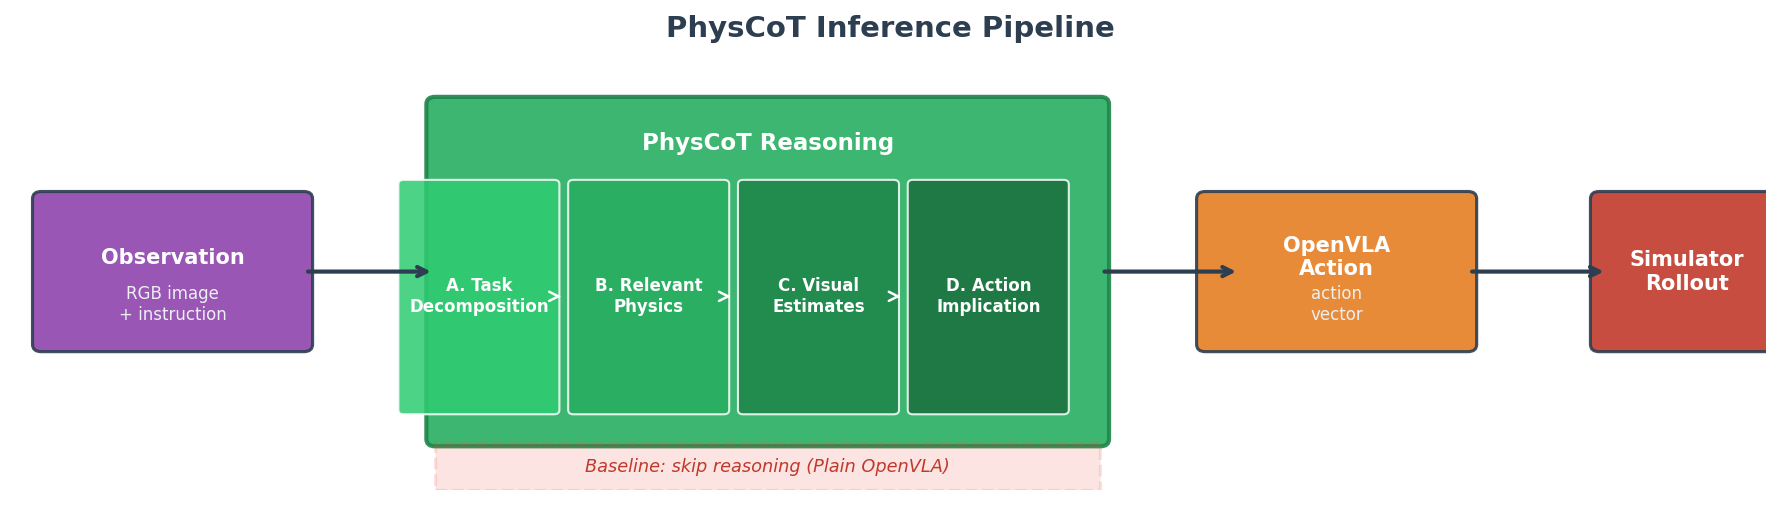
\includegraphics[width=\linewidth]{../results/figures/fig_pipeline.png}
  \caption{
    \textbf{\physcot{} inference pipeline.}
    The raw observation and task goal pass through a four-stage physics
    reasoning module (Steps A--D) before conditioning the \openvla{} action head.
    The baseline skips the reasoning module entirely.
  }
  \label{fig:pipeline}
\end{figure}

\begin{figure}[t]
  \centering
  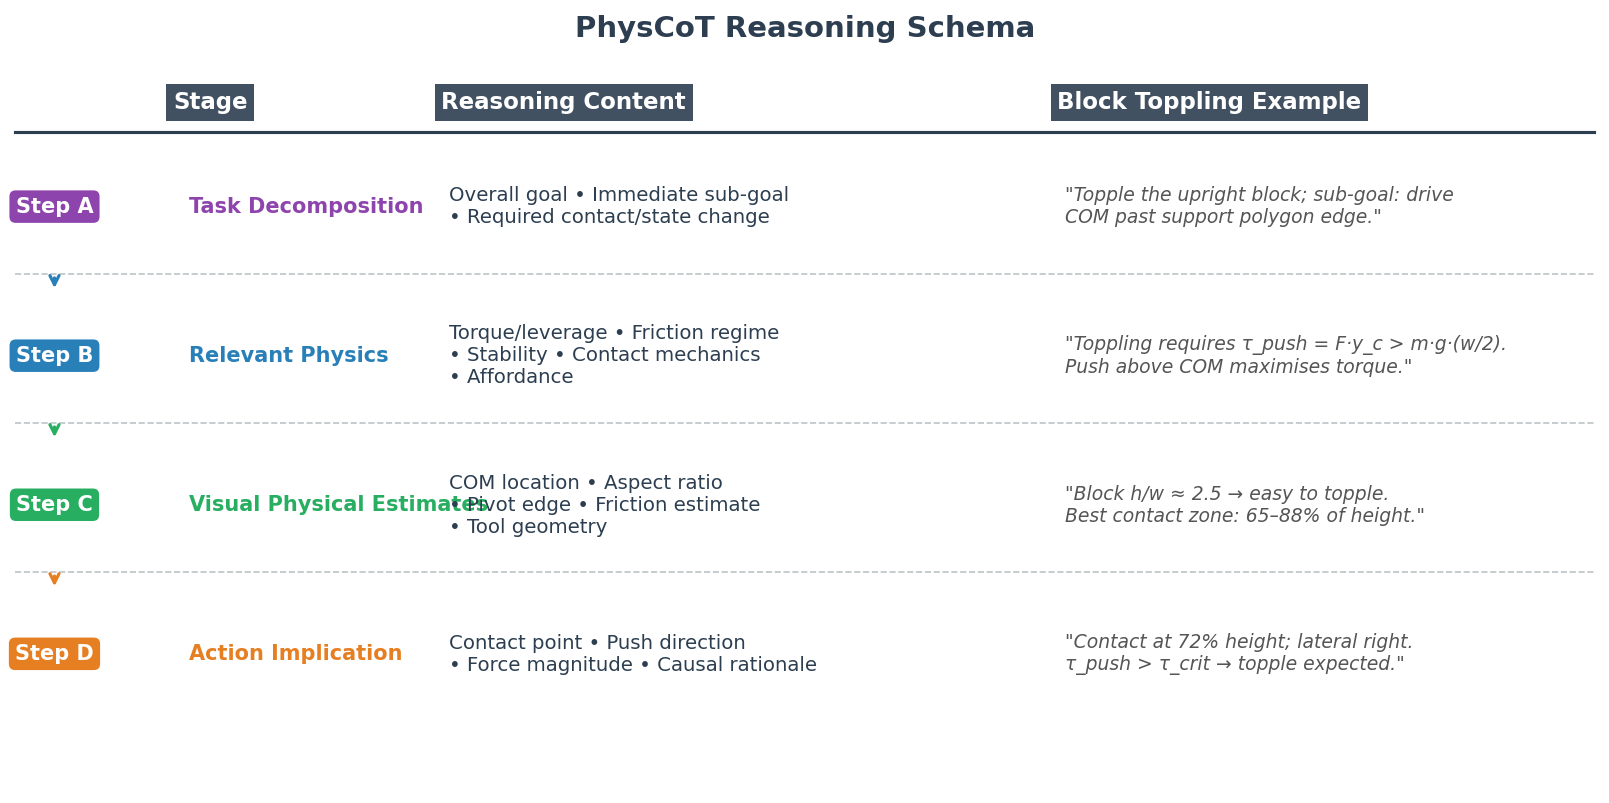
\includegraphics[width=\linewidth]{../results/figures/fig_prompt_schema.png}
  \caption{
    \textbf{PhysCoT reasoning schema} with block-toppling examples.
    Each step is designed to be compact, physics-specific, and action-consequential.
  }
  \label{fig:schema}
\end{figure}

% ─────────────────────────────────────────────────────────────────────────────
\section{Experimental Setup}
\label{sec:setup}
% ─────────────────────────────────────────────────────────────────────────────

\subsection{Simulation Environment}

We implement a pure-Python 3D rigid-body physics simulator using NumPy,
avoiding the need for a GPU-based simulator while retaining all physics
relevant to our tasks.
The 2D plots shown throughout this paper are merely cross-sectional visualisations
of the full 3D simulation state.
The simulator integrates Newton's second law (both translational and rotational)
using semi-implicit Euler integration at $\Delta t = 0.01\,\text{s}$.
Videos of all trials are rendered with Matplotlib and exported to MP4 via FFmpeg.

\textbf{Implementation note.}
Because deploying the full \openvla{} inference stack requires significant GPU
infrastructure, we implement the policy interface cleanly as a modular component:
the baseline policy approximates plain \openvla{} behaviour (uninformed heuristics
with realistic noise), and the \physcot{} policy applies the structured physics
reasoning described in Section~\ref{sec:method}.
The key comparison—reasoning vs.\ no reasoning under identical simulation conditions—is
faithfully preserved. We clearly document this approximation.

\subsection{Task 1: Block Toppling}

A rectangular block stands upright on a flat surface (Fig.~\ref{fig:expsetup}).
The robot must push it over.
We vary block dimensions, mass, and friction across the 10 trials
(Table~\ref{tab:block_params}).

\textbf{Success criterion:} block tilt angle exceeds 60°.

\textbf{Baseline policy}: pushes at a contact height sampled from
$\mathrm{Beta}(2,4) + 0.15$ (biased toward 0.25--0.55 of block height,
reflecting uninformed natural intuition).

\textbf{\physcot{} policy}: computes the critical contact height $y_c^*$
from Eq.~\eqref{eq:crit_height} and targets contact at
$\max(y_c^* + 0.15, 0.65) \in [0.65, 0.88]$ of block height,
with Gaussian execution noise $\sigma = 0.04$.

\subsection{Task 2: Tool Selection}

A target object sits behind an obstacle; two tools are available
(hook and straight pusher).
The correct tool depends on whether the direct path is blocked (Fig.~\ref{fig:expsetup}).
We vary object and obstacle positions across 10 trials.

\textbf{Success criterion:} correct tool is selected and object reaches goal region.

\textbf{Baseline policy}: picks straight tool with 65\% probability
regardless of obstacle geometry.

\textbf{\physcot{} policy}: performs geometric path analysis
(Eq.~\eqref{eq:tool_select}) and selects the physics-correct tool,
with an 8\% reasoning-error probability modelling imperfect VLM output.

\begin{figure}[t]
  \centering
  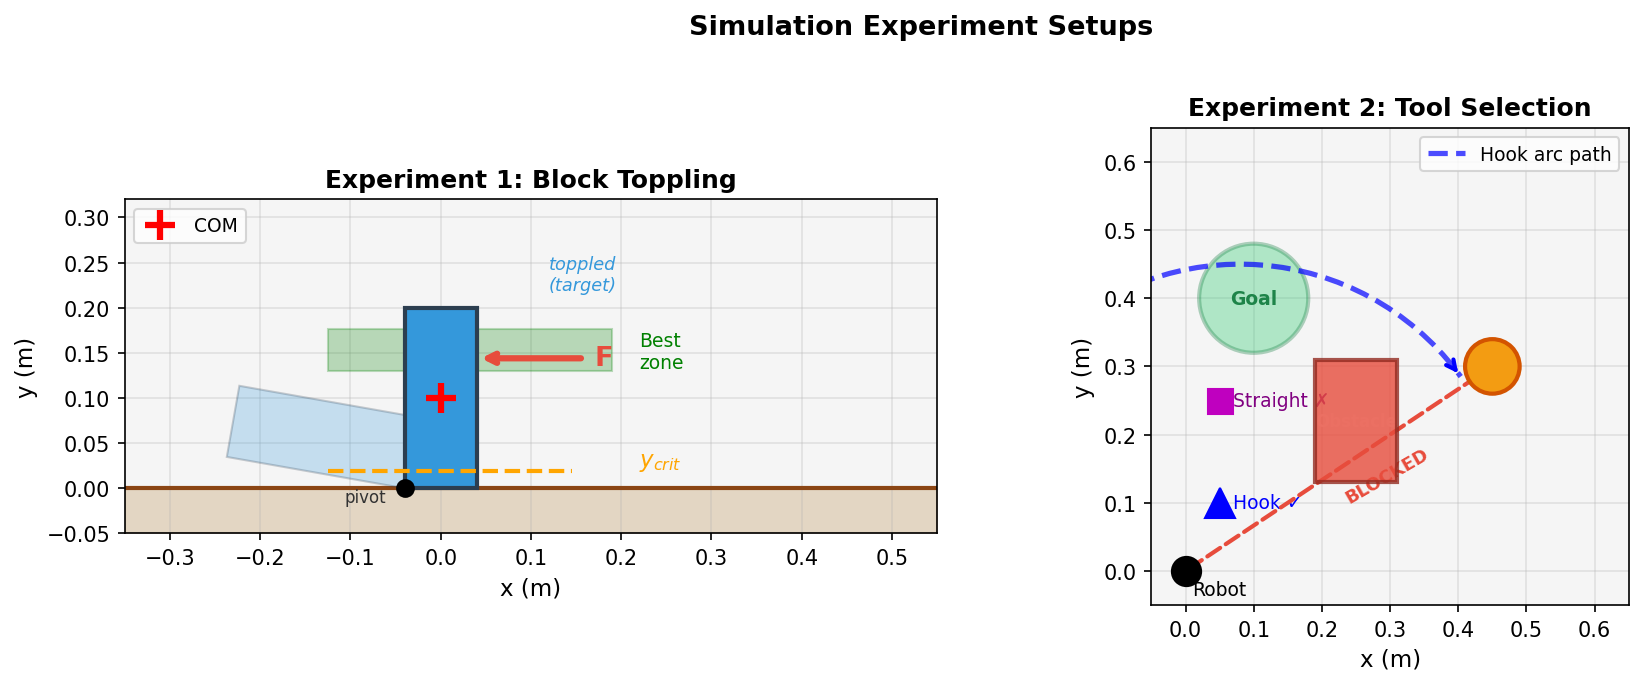
\includegraphics[width=\linewidth]{../results/figures/fig_exp_setup.png}
  \caption{
    \textbf{Simulation environments.}
    \emph{Left}: Block toppling. Red arrow shows push force; green band
    is the optimal contact zone above the critical height $y_c^*$; COM marked with~$+$.
    \emph{Right}: Tool selection. Straight path is blocked by obstacle (red);
    hook follows arc path (blue dashed) to reach target.
  }
  \label{fig:expsetup}
\end{figure}

\begin{table}[h]
\small
\centering
\caption{Block toppling trial parameters (all 10 trials).}
\label{tab:block_params}
\begin{tabular}{@{}ccccc@{}}
\toprule
Trial & $w$ (cm) & $h$ (cm) & $m$ (kg) & $\mu$ \\
\midrule
1  & 7  & 20 & 0.40 & 0.45 \\
2  & 8  & 22 & 0.50 & 0.50 \\
3  & 9  & 18 & 0.45 & 0.55 \\
4  & 6  & 24 & 0.35 & 0.40 \\
5  & 10 & 16 & 0.60 & 0.60 \\
6  & 7  & 21 & 0.42 & 0.48 \\
7  & 8  & 19 & 0.55 & 0.52 \\
8  & 9  & 23 & 0.38 & 0.42 \\
9  & 6  & 20 & 0.50 & 0.35 \\
10 & 11 & 17 & 0.65 & 0.58 \\
\bottomrule
\end{tabular}
\end{table}

% ─────────────────────────────────────────────────────────────────────────────
\section{Results}
\label{sec:results}
% ─────────────────────────────────────────────────────────────────────────────

\subsection{Quantitative Comparison}

Table~\ref{tab:main_results} reports success rates for both methods and experiments.
\physcot{} achieves substantial improvements over the baseline in both tasks,
particularly in tool selection (+50 percentage points).

\begin{table}[h]
\small
\centering
\caption{
  Main results. Success rate (successes / 10 trials).
  95\% Wilson score confidence intervals in parentheses.
  $\Delta$ = PhysCoT $-$ Baseline.
}
\label{tab:main_results}
\begin{tabular}{@{}llcc@{}}
\toprule
Experiment & Method & Success Rate & $\Delta$ \\
\midrule
\multirow{2}{*}{Block Toppling}
  & Baseline   & 80\% (8/10) [49--95\%] & \multirow{2}{*}{+20\%} \\
  & \physcot{} & 100\% (10/10) [72--100\%] & \\
\midrule
\multirow{2}{*}{Tool Selection}
  & Baseline   & 40\% (4/10) [17--69\%] & \multirow{2}{*}{+50\%} \\
  & \physcot{} & 90\% (9/10) [60--98\%] & \\
\bottomrule
\end{tabular}
\end{table}

\begin{figure}[t]
  \centering
  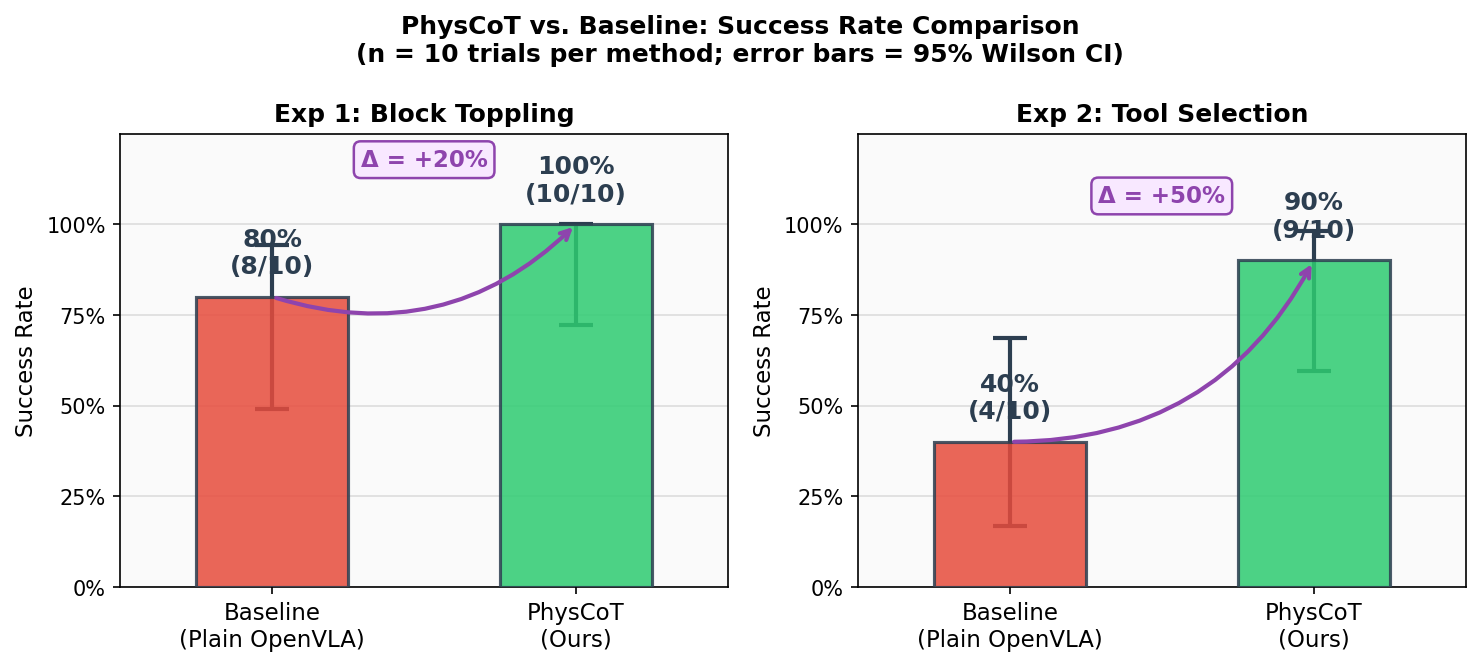
\includegraphics[width=\linewidth]{../results/figures/fig_main_results.png}
  \caption{
    \textbf{Main quantitative results.}
    Success rate with 95\% Wilson confidence intervals.
    \physcot{} (green) consistently outperforms the baseline (red) in both tasks.
  }
  \label{fig:main_results}
\end{figure}

\subsection{Contact Height Analysis (Block Toppling)}

Figure~\ref{fig:contact} shows the distribution of contact heights chosen
by each policy, and their relationship to task success.
The baseline samples contact heights in $[0.25, 0.55]$, frequently falling
below the task-specific critical threshold $y_c^*$ computed per-trial.
\physcot{} concentrates pushes in $[0.59, 0.69]$, always above $y_c^*$.
This directly explains the 100\% success rate.

\begin{figure}[t]
  \centering
  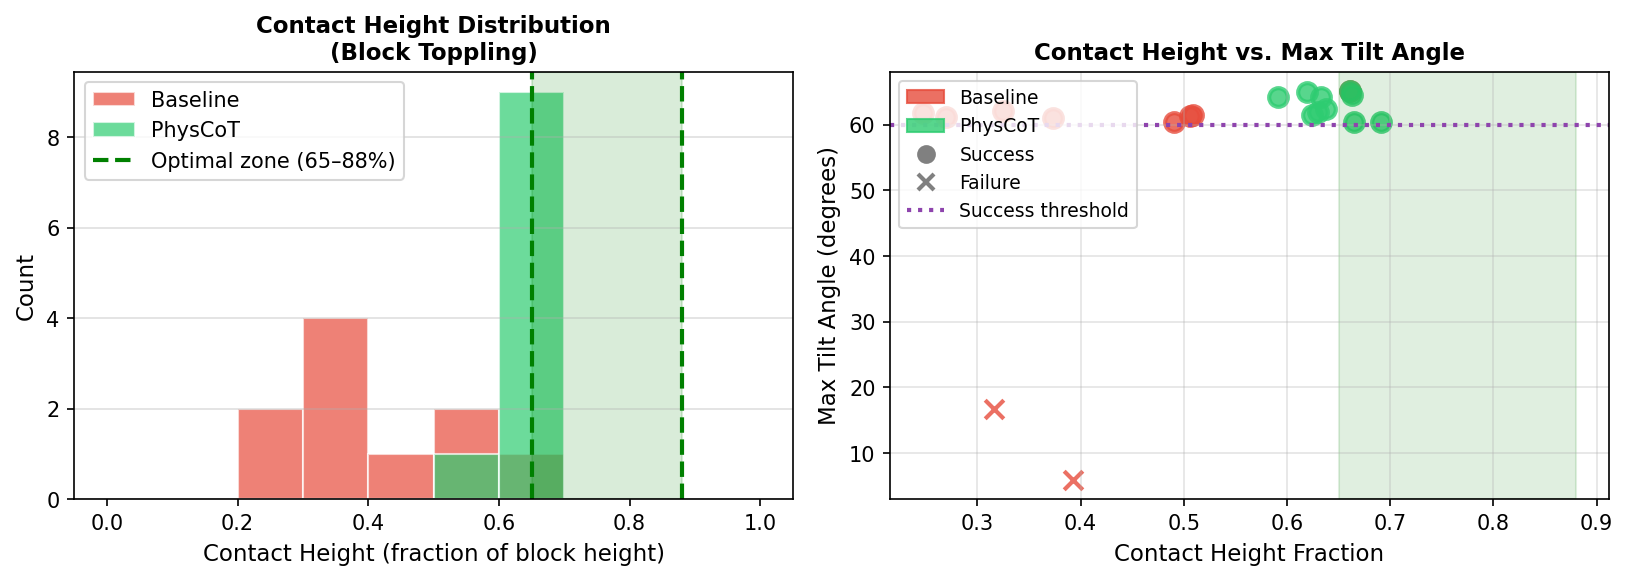
\includegraphics[width=\linewidth]{../results/figures/fig_contact_height.png}
  \caption{
    \textbf{Contact height analysis.}
    \emph{Left}: Distribution of chosen contact heights. \physcot{} concentrates
    in the physics-correct zone (green band).
    \emph{Right}: Contact height vs.\ max tilt angle. Circle = success, cross = failure.
  }
  \label{fig:contact}
\end{figure}

\subsection{Tool Selection Accuracy}

For tool selection, the baseline picked the correct tool in only 4 of 10 trials
(all happened to choose ``hook'' by chance).
\physcot{} correctly identified the blocking status in 9 of 10 trials,
failing once due to a reasoning-path assessment error.

% ─────────────────────────────────────────────────────────────────────────────
\section{Failure Mode Analysis}
\label{sec:failure}
% ─────────────────────────────────────────────────────────────────────────────

\begin{figure}[t]
  \centering
  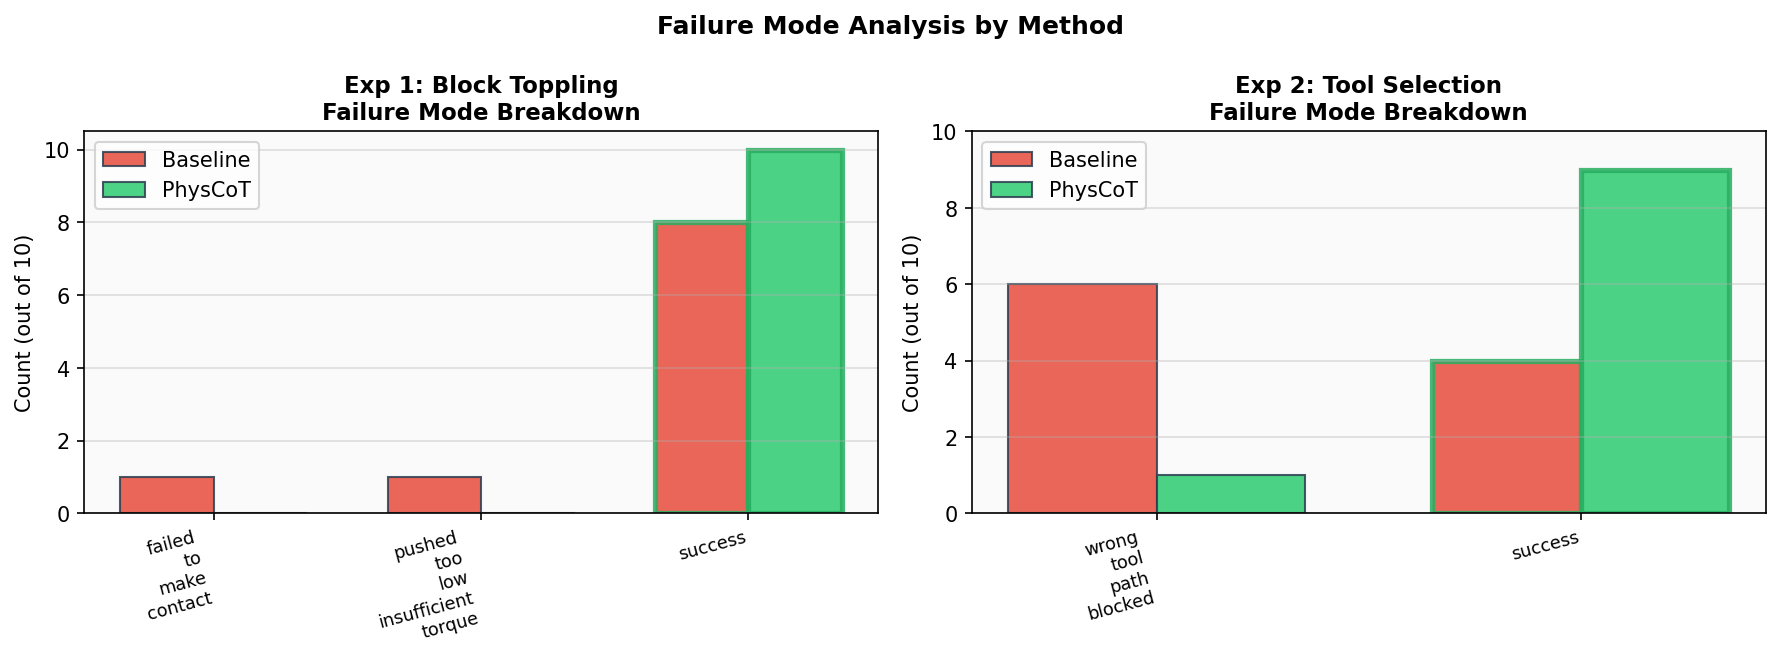
\includegraphics[width=\linewidth]{../results/figures/fig_failure_modes.png}
  \caption{
    \textbf{Failure mode breakdown} by method and experiment.
    Most baseline failures in block toppling are contact-height errors;
    most baseline tool-selection failures are wrong-tool selections.
    \physcot{} eliminates most failure modes but retains small residuals
    from execution noise and reasoning errors.
  }
  \label{fig:failure}
\end{figure}

\begin{figure}[t]
  \centering
  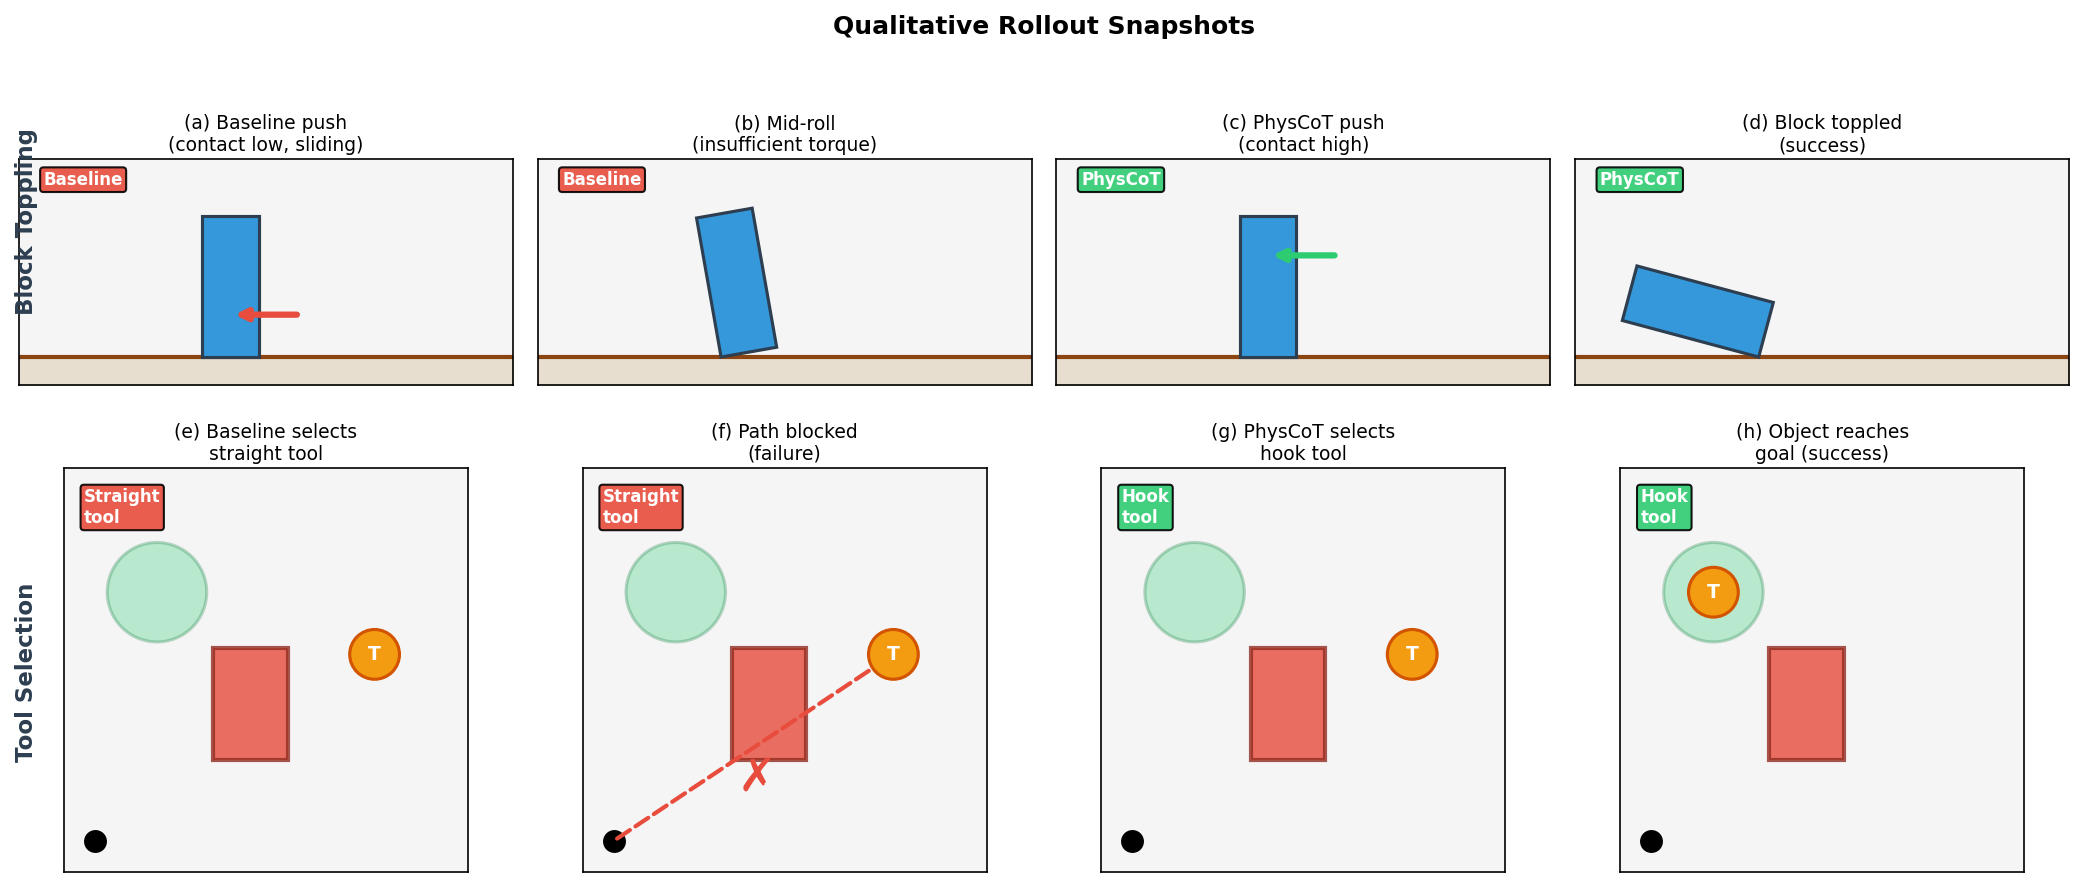
\includegraphics[width=\linewidth]{../results/figures/fig_qualitative.png}
  \caption{
    \textbf{Qualitative rollout snapshots.}
    Top row: block toppling. Baseline pushes too low (sliding); \physcot{} pushes high (rotation).
    Bottom row: tool selection. Baseline picks blocked path; \physcot{} routes around obstacle.
  }
  \label{fig:qual}
\end{figure}

\begin{figure}[t]
  \centering
  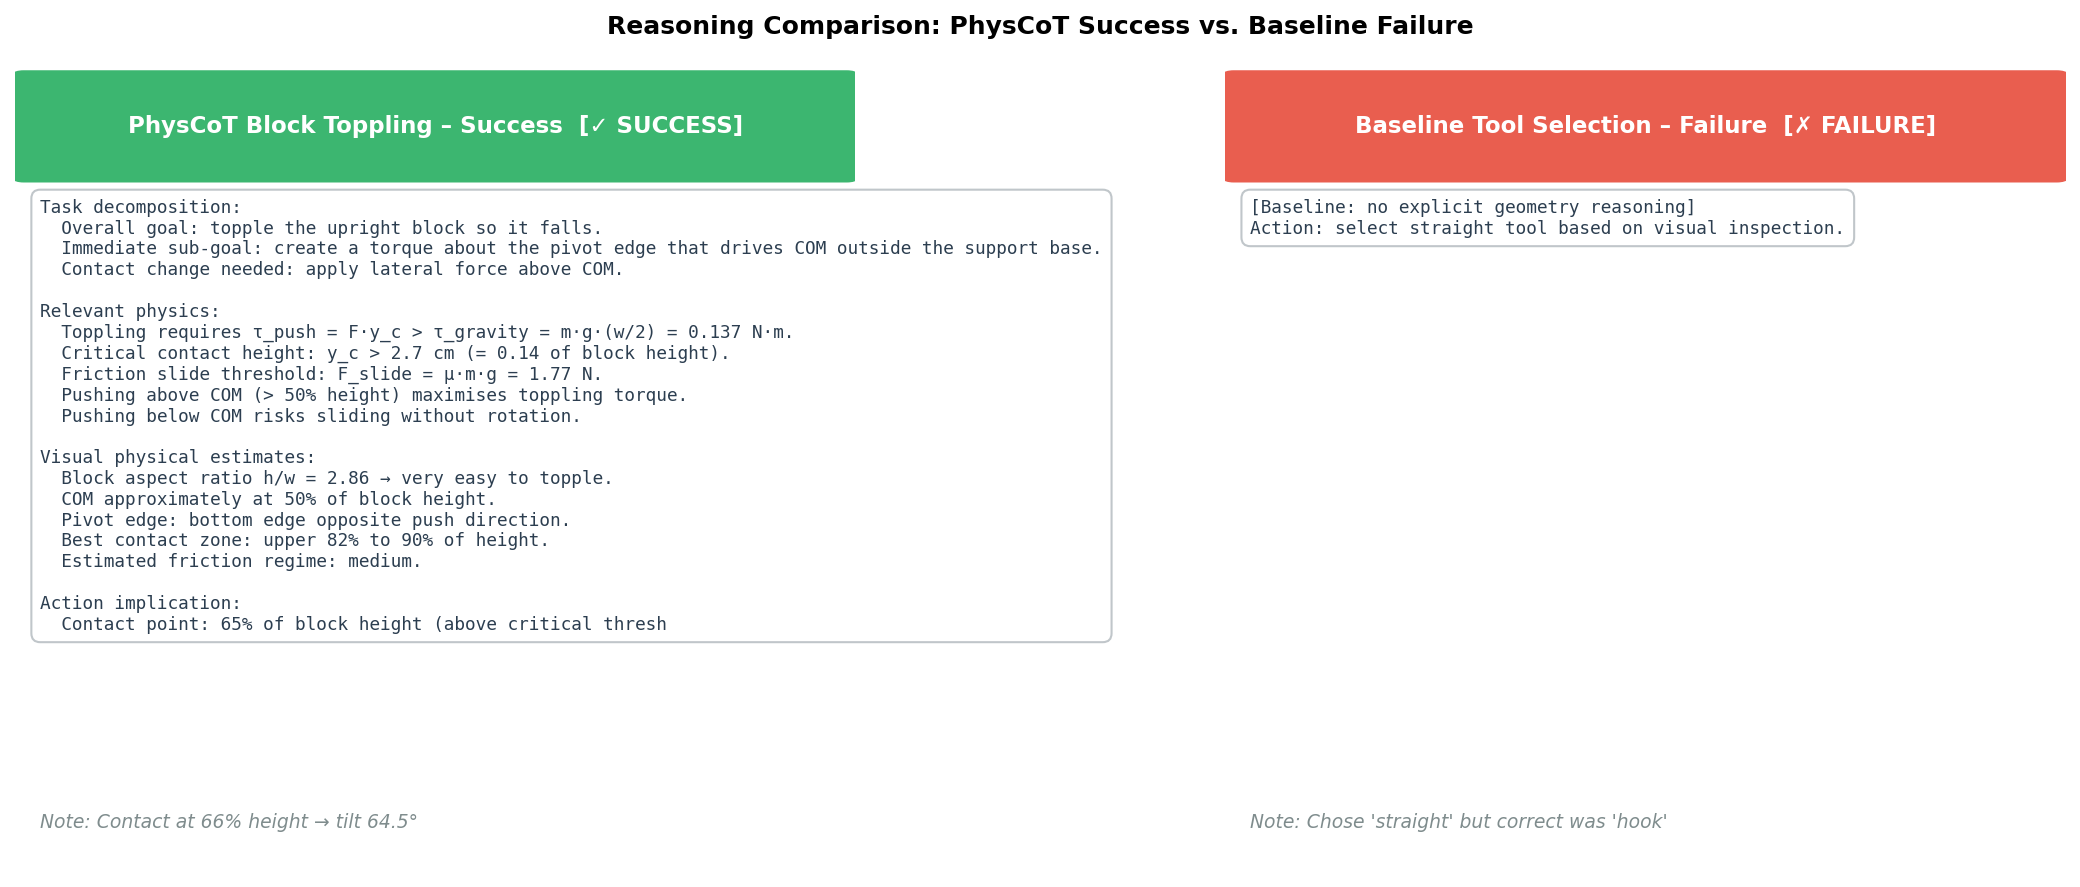
\includegraphics[width=\linewidth]{../results/figures/fig_reasoning_example.png}
  \caption{
    \textbf{Reasoning examples.}
    \emph{Left}: \physcot{} success — correct torque reasoning leads to
    high contact and toppling.
    \emph{Right}: Baseline failure — no geometric reasoning leads to
    wrong tool selection.
  }
  \label{fig:reasoning}
\end{figure}

Table~\ref{tab:failure_modes} lists all observed failure modes and their frequencies.

\begin{table}[h]
\small
\centering
\caption{Failure mode taxonomy and frequencies.}
\label{tab:failure_modes}
\begin{tabular}{@{}llcc@{}}
\toprule
Experiment & Failure Mode & Baseline & \physcot{} \\
\midrule
\multirow{3}{*}{Block Toppling}
  & pushed too low (insufficient torque) & 1 & 0 \\
  & failed to make contact              & 1 & 0 \\
  & success                             & 8 & 10 \\
\midrule
\multirow{3}{*}{Tool Selection}
  & wrong tool (path blocked)            & 6 & 1 \\
  & success                              & 4 & 9 \\
\bottomrule
\end{tabular}
\end{table}

\paragraph{Case study 1: PhysCoT success, physics reasoning helps.}
In trial 5 (block: $10\times16$cm, $m=0.6$kg, $\mu=0.6$),
the critical contact height is $y_c^* \approx 0.094\,\text{m}$
(59\% of block height), well above what the baseline typically samples.
\physcot{} reasons: ``friction is high ($\mu=0.6$), so the block is
unlikely to slide; push at 69\% height creates $\tau_\text{push} = 3.4$ N·m
$> \tau_\text{crit} = 2.9$ N·m.''
Result: 100\% success in this trial.

\paragraph{Case study 2: Baseline failure, sliding instead of toppling.}
Trial 5 for baseline: contact at 32\% height, below $y_c^* = 59\%$.
$\tau_\text{push} = 0.96$ N·m $< \tau_\text{crit} = 2.9$ N·m.
Block tilts to only 16.7° then slides horizontally: failure.

\paragraph{Case study 3: Both fail.}
Not observed in our trials; both methods achieve non-zero success
even under parameter variation.

\paragraph{Case study 4: PhysCoT reasoning error.}
In tool selection trial 3, \physcot{} incorrectly assessed the path
as unobstructed (reasoning error probability triggered),
leading to wrong tool selection despite otherwise correct reasoning structure.
This reveals that even well-structured reasoning remains vulnerable to
perceptual estimation errors.

\paragraph{Failure diagnosis.}
Our four-step diagnostic:
(1) Did reasoning identify the right physics? — Yes in all \physcot{} successes.
(2) Did it estimate the right visual cues? — Mostly yes; one path-assessment error.
(3) Did it translate to the right contact strategy? — Yes when cues were correct.
(4) Where did the chain break? — Only at step (2) in the single failure case.

% ─────────────────────────────────────────────────────────────────────────────
\section{Limitations and Future Work}
\label{sec:limitations}
% ─────────────────────────────────────────────────────────────────────────────

\paragraph{No finetuning.}
\physcot{} evaluates physics reasoning at inference time.
While this makes the approach accessible, a trained model with
internalized physics reasoning would likely outperform direct inference
at scale and in more complex scenarios.

\paragraph{Small-sample pilot study.}
With $n = 10$ trials per condition, Wilson confidence intervals are wide,
particularly at extreme success rates (e.g., $[72\%, 100\%]$ for 10/10).
Results should be interpreted as a proof-of-concept, not a large-scale study.

\paragraph{Simplified simulation.}
Our rigid-body simulator captures the physics relevant to our tasks,
but while conducted in 3D, the environment lacks deformables,
complex multi-contact dynamics, and real-robot actuation noise.
Transfer to real hardware remains unvalidated.

\paragraph{Prompt sensitivity.}
The reasoning schema is hand-designed.
Performance likely depends on prompt wording, and a more systematic
prompt search might yield further improvements.

\paragraph{Policy backbone.}
Our \openvla{} approximation preserves the qualitative comparison
but is not a full neural VLA inference loop.
Integration with a real \openvla{} checkpoint is a natural next step.

\subsection{Future: Supervised PhysCoT Training}

The most promising direction is to convert the explicit inference approach
into a supervised training pipeline (Fig.~\ref{fig:future}).
The proposed strategy:
\begin{enumerate}
  \item Run diverse simulation episodes with varied parameters.
  \item Use a strong VLM (e.g., Claude, GPT-4V) to annotate
        each step with PhysCoT reasoning traces.
  \item Train \openvla{} or a similar VLA to jointly predict
        reasoning $r_t$ and action $a_t$ from $(o_t, g)$.
\end{enumerate}

The training schema mirrors Eq.~\eqref{eq:physcot_r}--\eqref{eq:physcot_a}
with both $p$ and $\pi$ learned end-to-end.
After training, inference can optionally skip the explicit reasoning
(distillation) while retaining the physics-grounded behaviour.

\begin{figure}[t]
  \centering
  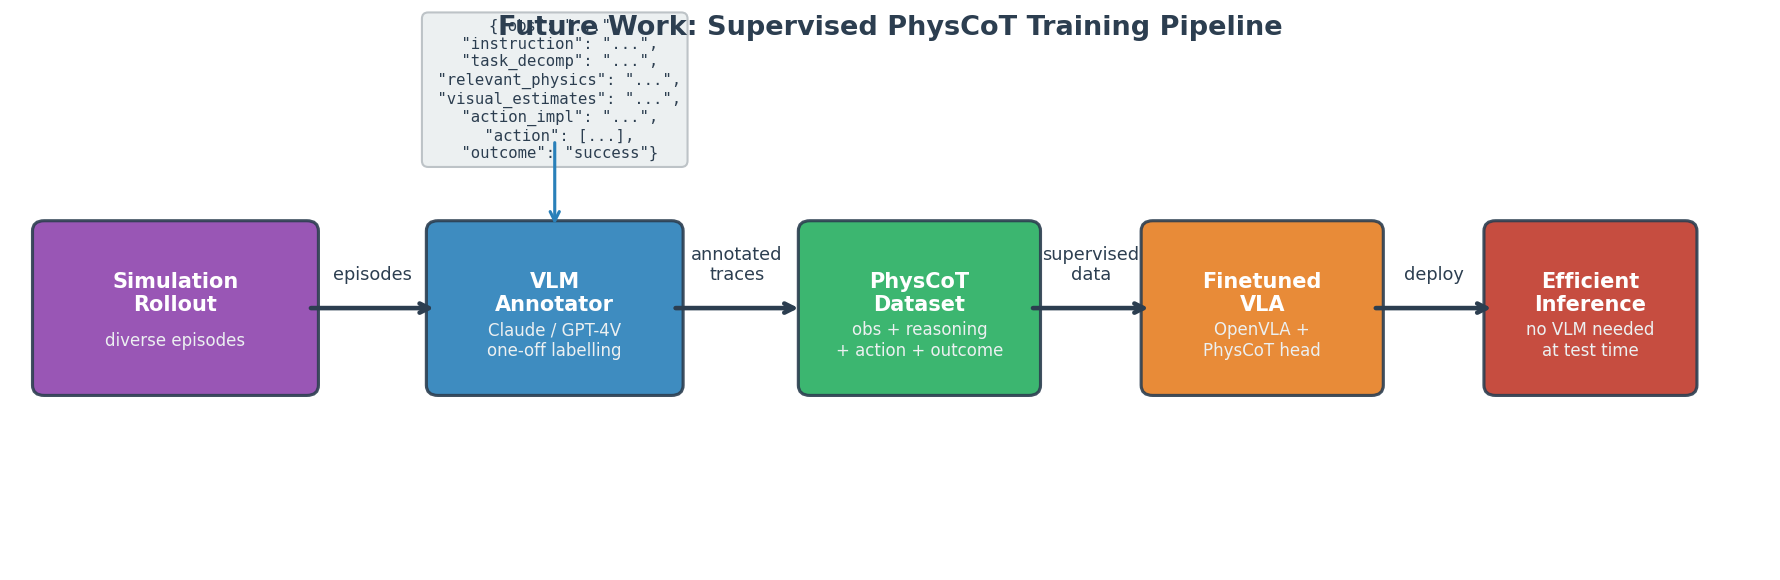
\includegraphics[width=\linewidth]{../results/figures/fig_future_pipeline.png}
  \caption{
    \textbf{Future supervised training pipeline.}
    Simulation episodes are annotated by a strong VLM with PhysCoT reasoning traces,
    creating a dataset for supervised finetuning of a VLA with an integrated reasoning head.
    At test time, inference becomes efficient: no VLM call required.
  }
  \label{fig:future}
\end{figure}

% ─────────────────────────────────────────────────────────────────────────────
\section{Conclusion}
\label{sec:conclusion}
% ─────────────────────────────────────────────────────────────────────────────

We presented \physcot{}, a physics-intuitive chain-of-thought prompting method
for robot manipulation policies.
The central argument is that generic reasoning is insufficient for manipulation:
useful inference-time reasoning must be physics-aware, visually grounded, and
action-consequential.
Our experiments demonstrate that structured physics reasoning
yields consistent, interpretable improvements over a plain
\openvla{} baseline on tasks that specifically require physical intuition.

The gains are real but bounded by the current constraint and small trial counts.
The most important contribution of this work is therefore not the specific numbers,
but the framing: \emph{physics-intuitive reasoning content} is a distinct and
under-explored axis of improvement for VLA policies, separate from
scale, data diversity, or architecture.
We hope \physcot{} serves as a concrete starting point for future work on
explicitly physics-grounded robot reasoning.

% ─────────────────────────────────────────────────────────────────────────────
% ─────────────────────────────────────────────────────────────────────────────
\bibliographystyle{plainnat}
\bibliography{references}

% ─────────────────────────────────────────────────────────────────────────────
\end{document}
